\documentclass[conference]{IEEEtran}
\IEEEoverridecommandlockouts

\usepackage{cite}
\usepackage{amsmath,amssymb,amsfonts}
\usepackage{graphicx}
\usepackage{booktabs}
\usepackage{multirow}
\usepackage{xcolor}
\usepackage{pifont}
\usepackage{url}
\usepackage[hidelinks]{hyperref}

\graphicspath{{figures/panels/}}

\newcommand{\cmark}{{\color{green!60!black}\ding{51}}}
\newcommand{\xmark}{{\color{red}\ding{55}}}

\begin{document}

\title{Post-hoc Entropy Minimization Improves\\ Semi-Supervised Medical Image Segmentation}

\author{
\IEEEauthorblockN{Tal Shaharabany}
\IEEEauthorblockA{\textit{Blavatnik School of Computer Science}\\
\textit{Tel Aviv University}\\
Tel Aviv, Israel\\
shaharabany@mail.tau.ac.il}
\and
\IEEEauthorblockN{Natalie Carlebach}
\IEEEauthorblockA{\textit{Tel Aviv University}\\
Tel Aviv, Israel\\
nataliecarlebach@gmail.com}
\and
\IEEEauthorblockN{Lior Wolf}
\IEEEauthorblockA{\textit{Blavatnik School of Computer Science}\\
\textit{Tel Aviv University}\\
Tel Aviv, Israel\\
wolf@cs.tau.ac.il}
}

\maketitle

\begin{abstract}
Semi-supervised learning (SSL) methods for medical image segmentation stop using the unlabeled data once training converges, even though the model's predictions on it still carry residual uncertainty concentrated at organ boundaries. We show that this residual entropy is spatially structured and exploit it with \textit{Post-hoc Entropy Minimization} (PEM): any converged SSL checkpoint is fine-tuned for two to five epochs with a single entropy-minimization loss on unlabeled data, using no labels, no pseudo-labels, and no architectural changes. Applied to the publicly released Bidirectional Copy-Paste (BCP) checkpoints with no test-set tuning, PEM improves the Dice score by $+1.12$, $+1.43$, and $+0.64$ points on Pancreas-CT (20\% labeled), Left Atrium (5\% labeled), and Left Atrium (10\% labeled), respectively, and reduces the 95th-percentile Hausdorff Distance by $27$--$43\%$, in under five minutes per run on a single GPU. Against three controlled post-hoc baselines --- temperature scaling, pseudo-label fine-tuning, and self-consistency --- PEM obtains the largest mean gain on the two less-saturated configurations, and every gain passes a per-case Wilcoxon signed-rank test ($p<0.025$).
\end{abstract}

\begin{IEEEkeywords}
semi-supervised learning, medical image segmentation, entropy minimization, post-hoc fine-tuning
\end{IEEEkeywords}

\section{Introduction}
\label{sec:intro}
Manual voxel-level annotation of 3D medical scans is slow and expensive, which makes semi-supervised learning (SSL) --- training from a small labeled set together with a large unlabeled set --- a practical necessity for volumetric segmentation. Recent SSL methods for this task~\cite{tarvainen2017meanteacher,yu2019uamt,bai2023bcp,liu2024most,assefa2025dycon} reach strong accuracy by using the unlabeled data during training and then discarding it at convergence.

We make a complementary observation: at convergence, a well-trained SSL model still assigns non-trivial prediction entropy to the unlabeled volumes, and this entropy is not uniformly spread. It is concentrated in a thin shell of low-confidence voxels lying on the predicted organ boundary. This concentration is a property of SSL convergence rather than of any single method, and it is exactly the condition under which a label-free sharpening step is well-behaved: the loss gradient it produces is already aligned with the locus of segmentation error.

We exploit this with \textit{Post-hoc Entropy Minimization} (PEM). Given any converged SSL checkpoint, PEM fine-tunes it for a few epochs on the unlabeled data with a single entropy-minimization objective. It requires no labels, no pseudo-labels, no thresholds, and no changes to the network. It runs in minutes on one GPU and can be applied on top of a released checkpoint without retraining. Entropy minimization itself is classical~\cite{grandvalet2004entropy,sohn2020fixmatch}; our contribution is identifying its correct \textit{operating regime} --- a converged optimum whose residual entropy is already structurally concentrated --- and showing that in this regime the same loss needs no masking, curriculum, or class-balance regularizer.

\noindent\textbf{Contributions.}
\begin{itemize}
\item We introduce a label-free diagnostic, the \textit{shell entropy concentration} $\rho_f(\tau)$, that measures what fraction of a model's total prediction entropy is carried by its low-confidence voxels, and we use it to characterize when post-hoc sharpening is expected to help.
\item We propose PEM, a simple post-hoc fine-tuning step that improves any converged SSL checkpoint on unlabeled data alone, and we relate its gradient to the cluster assumption at the organ surface.
\item On three public SSL checkpoints spanning two organs and two modalities, PEM consistently improves overlap and boundary metrics, and outperforms three controlled post-hoc baselines under an identical fixed-budget protocol with no test-set tuning.
\end{itemize}

\section{Related Work}
\label{sec:related}
\noindent\textbf{SSL for medical image segmentation.}
Most recent methods build on the Mean Teacher framework~\cite{tarvainen2017meanteacher}, in which a student network is trained to agree with a teacher whose weights are an exponential moving average (EMA) of the student's. Uncertainty-Aware Mean Teacher (UA-MT)~\cite{yu2019uamt} filters the consistency target by estimated uncertainty. Bidirectional Copy-Paste (BCP)~\cite{bai2023bcp} mixes labeled and unlabeled crops in both directions to align their distributions and is a strong, widely used baseline. More recent methods such as MOST~\cite{liu2024most} and DyCON~\cite{assefa2025dycon} further improve accuracy but release training code only. All of these approaches use the unlabeled data only during training.

\noindent\textbf{Entropy minimization and test-time adaptation.}
Entropy minimization~\cite{grandvalet2004entropy} encourages confident predictions on unlabeled data and underlies consistency-based SSL objectives~\cite{sohn2020fixmatch}. Test-time entropy minimization (TENT) adapts a model to a shifted test distribution by minimizing prediction entropy over its outputs. PEM differs in regime and target: it is applied \textit{after} SSL convergence, on the same unlabeled training distribution rather than a shifted test set, and it updates all parameters rather than only normalization statistics. As we show, applying entropy minimization at a converged optimum whose residual entropy is already concentrated on the boundary shell is what removes the need for the masks and regularizers that entropy-based objectives normally require.

\section{Method}
\label{sec:method}
\subsection{Shell Entropy Concentration}
Let $f_{\theta^*}$ be a converged checkpoint and $\mathbf{x}\in\mathcal{U}$ an unlabeled volume. For voxel $i$ with per-class softmax probabilities $p_{i,c}$, define the per-voxel entropy $H_i=-\sum_c p_{i,c}\log p_{i,c}$ and confidence $c_i=\max_c p_{i,c}$. The \textit{shell entropy concentration} at confidence threshold $\tau$ is
\begin{equation}
\rho_f(\tau) \;=\; \frac{\mathbb{E}_{\mathbf{x}\sim\mathcal{U}}\!\left[\sum_{i} H_i\,\mathbb{1}[c_i\le\tau]\right]}{\mathbb{E}_{\mathbf{x}\sim\mathcal{U}}\!\left[\sum_{i} H_i\right]} \in [0,1].
\label{eq:rho}
\end{equation}
$\rho_f(\tau)$ is the fraction of total prediction entropy carried by voxels of confidence at most $\tau$. It is label-free, scalar, and self-localizing: on a converged network the low-confidence voxels lie near the decision boundary. We use $\tau=0.99$ throughout and treat $\rho^\star=0.85$ as a suitability threshold, above which post-hoc sharpening is expected to help.

\subsection{Post-hoc Entropy Minimization}
PEM fine-tunes the checkpoint on the unlabeled set with the entropy loss
\begin{equation}
\mathcal{L}_{\text{PEM}} \;=\; \frac{1}{|\mathcal{U}|}\sum_{\mathbf{x}\in\mathcal{U}}\frac{\sum_{i} m_i H_i}{\sum_i m_i+\epsilon},
\qquad m_i=\mathbb{1}[c_i\le\tau],
\label{eq:pem}
\end{equation}
optionally restricted to the confidence shell through the mask $m_i$. No labels or pseudo-labels are used. Fine-tuning runs for a small, fixed number of epochs $E$ with a small learning rate.

\subsection{Why the Regime Matters}
Consider a binary voxel with logit $z$ and probability $p=\sigma(z)$. Its entropy gradient is $\partial H/\partial z=-z\,p(1-p)$: the update vanishes as $p\to0$ or $p\to1$ and peaks at $p=0.5$. The factor $p(1-p)$ therefore acts as an implicit boundary-shell mask equivalent to $m_i$, so on a saturated network no explicit class-balance regularizer is needed. Because the feature-space decision surface co-locates with the organ surface in 3D segmentation, PEM implements the cluster assumption~\cite{chapelle2006ssl,grandvalet2004entropy} at the organ boundary. When residual entropy is instead diffuse ($\rho_f\lesssim0.6$), the same sharpening reinforces existing errors, which is why $\rho_f$ predicts applicability.

\section{Datasets and Implementation}
\label{sec:data}
\noindent\textbf{Datasets.}
We evaluate on two public benchmarks. Pancreas-CT~\cite{roth2015pancreas} contains abdominal Computed Tomography (CT) scans; following the standard split we use 12 labeled, 50 unlabeled, and 18 test cases (20\% labeled). The Left Atrium (LA) 2018 dataset contains cardiac Magnetic Resonance Imaging (MRI) scans; we use the standard 5\% (4 labeled) and 10\% (8 labeled) splits with 20 test cases. Both use the preprocessing distributed with BCP~\cite{bai2023bcp}.

\noindent\textbf{Checkpoints and protocol.}
We start from the publicly released BCP checkpoints (V-Net backbone; instance normalization for Pancreas, batch normalization for LA). PEM uses Adam (no weight decay, no schedule) with gradient clipping at $1$ and learning rates of $5\times10^{-5}$ (Pancreas) and $1\times10^{-5}$ (LA), selected by 5-fold cross-validation on the labeled folds only; LA batch-normalization statistics are frozen. The epoch budget is fixed \textit{a priori} at $E=2$ (Pancreas) and $E=5$ (LA). Reported PEM numbers are the mean over seeds $\{2020,42,123\}$. Inference uses sliding windows with BCP's original strides and no test-time augmentation (TTA); each PEM run completes in under $5.2$ minutes on a single RTX 4070 Ti SUPER.

\noindent\textbf{Metrics.}
We report the Dice score and Jaccard index (higher is better), and the 95th-percentile Hausdorff Distance (HD95) and Average Surface Distance (ASD) in voxels (lower is better).

\noindent\textbf{Post-hoc baselines.}
We compare PEM against three post-hoc methods that receive the same checkpoint, budget, learning rate, and data.
\textit{Temperature Scaling} (TS) fits a single scalar temperature $T$ on unlabeled entropy and cannot change the argmax prediction.
\textit{Pseudo-Label Fine-Tuning} (PL-FT) generates hard pseudo-labels (argmax followed by the largest connected component, CC) and fine-tunes with a cross-entropy plus Dice loss.
\textit{Self-Consistency} (SC) minimizes the mean-squared error between the student on a noised input and the frozen teacher on the clean input.
We compare against BCP because MOST~\cite{liu2024most} and DyCON~\cite{assefa2025dycon} release training code only.

\section{Experiments and Results}
\label{sec:experiments}
\noindent\textbf{Residual entropy is concentrated (Table~\ref{tab:entropy}).}
On the unlabeled training volumes, the three released BCP checkpoints carry $89$--$95\%$ of their total prediction entropy in a thin shell of only $5$--$9\%$ of the voxels, giving $\rho_f(0.99)\in\{0.894,0.948,0.945\}$. A supervised-only V-Net trained on the same 12 Pancreas-CT labels carries only $55\%$ of its entropy in the corresponding shell ($\rho_f=0.552$), and its uncertain voxels lie on average $14.5$ voxels from any boundary (versus $5$--$11$ voxels for the SSL checkpoints). This $34$--$40$ percentage-point gap is the precondition PEM relies on: all three SSL checkpoints clear $\rho^\star=0.85$, whereas the supervised baseline does not.

\begin{table}[t]
\centering
\caption{Shell entropy concentration $\rho_f(\tau)$ on unlabeled training volumes. \textbf{Sat\%}: fraction of voxels with $c_i>0.99$. $\bar d$: mean distance from uncertain voxels to the predicted boundary (voxels). The three SSL checkpoints clear $\rho^\star{=}0.85$; the supervised baseline does not.}
\label{tab:entropy}
\footnotesize
\setlength{\tabcolsep}{4pt}
\begin{tabular}{lcccc}
\toprule
\textbf{Checkpoint} & \textbf{Sat\%} & \textbf{Unc\%} & $\boldsymbol{\rho_f(0.99)}$ & $\bar d$ \\
\midrule
Supervised V-Net (no SSL)   & 90.7 & 9.3 & 0.552~\xmark & 14.45 \\
BCP Pancreas-CT 20\%        & \textbf{95.0} & 5.0 & \textbf{0.894}~\cmark & 10.56 \\
BCP LA 5\%                  & 91.8 & 8.2 & \textbf{0.948}~\cmark & ~5.19 \\
BCP LA 10\%                 & 91.4 & 8.6 & \textbf{0.945}~\cmark & ~5.96 \\
\bottomrule
\end{tabular}
\end{table}

\noindent\textbf{PEM improves every checkpoint (Table~\ref{tab:main}).}
TS produces $|\Delta\text{Dice}|\le0.03$ on all settings, confirming that PEM's gain comes from parameter updates at boundary voxels rather than recalibration; we therefore omit its row. PEM attains the largest Dice and HD95 improvement on the two less-saturated configurations ($+1.12$ and $+1.43$ Dice, versus $+0.50$ and $+1.09$ for PL-FT). On the most saturated setting, LA 10\% (BCP at $89.40$), PL-FT marginally exceeds PEM ($+0.80$ versus $+0.64$) with overlapping bootstrap confidence intervals --- consistent with the soft $p(1-p)$ gradient shrinking as $\rho_f\to1$. Across three seeds PEM is stable ($84.01\pm0.00$, $88.59\pm0.25$, $90.02\pm0.07$), and a per-case paired analysis ($N=18$--$20$; Wilcoxon $p<0.025$; confidence-interval lower bound $\ge+0.18$; effect size $d_z\in[0.57,0.71]$; $13$--$16$ wins) confirms the gain on all three settings. Fig.~\ref{fig:qual} shows the boundary sharpening qualitatively.

\begin{table}[t]
\centering
\caption{Post-hoc methods on the released BCP checkpoints under an identical fixed-budget protocol. TS omitted (Dice change $|\Delta|{\le}0.03$ everywhere). Boldface marks the best Dice per setting. PEM wins the two less-saturated configurations and overlaps PL-FT (confidence interval) on the saturated LA 10\%.}
\label{tab:main}
\footnotesize
\setlength{\tabcolsep}{3.5pt}
\begin{tabular}{lcccc}
\toprule
\textbf{Method} & \textbf{Dice}$\uparrow$ & \textbf{Jaccard}$\uparrow$ & \textbf{HD95}$\downarrow$ & \textbf{ASD}$\downarrow$ \\
\midrule
\multicolumn{5}{l}{\textit{Pancreas-CT 20\% \; (12L / 50U / 18T)}} \\
BCP (released ckpt)          & 82.89 & 71.01 &  7.81 & 2.62 \\
\quad$+$ PL-FT               & 83.39 & 71.76 &  7.75 & 2.37 \\
\quad$+$ SC                  & 83.10 & 71.31 &  7.38 & 2.47 \\
\quad$+$ \textbf{PEM (ours)} & \textbf{84.01} & \textbf{72.66} & \textbf{5.71} & \textbf{1.68} \\
\midrule
\multicolumn{5}{l}{\textit{LA 5\% \; (4L / 76U / 20T)}} \\
BCP (released ckpt)          & 87.32 & 77.65 & 13.91 & 3.60 \\
\quad$+$ PL-FT               & 88.22 & 79.02 &  8.67 & 2.41 \\
\quad$+$ SC                  & 88.03 & 78.71 & 10.10 & 2.83 \\
\quad$+$ \textbf{PEM (ours)} & \textbf{88.59} & \textbf{79.62} & \textbf{7.98} & \textbf{1.98} \\
\midrule
\multicolumn{5}{l}{\textit{LA 10\% \; (8L / 72U / 20T)}} \\
BCP (released ckpt)          & 89.40 & 80.92 &  9.88 & 2.86 \\
\quad$+$ \textbf{PL-FT}      & \textbf{90.08} & \textbf{82.02} & \textbf{6.37} & \textbf{1.86} \\
\quad$+$ SC                  & 89.42 & 81.01 &  7.85 & 2.24 \\
\quad$+$ PEM (ours)          & 90.02 & 81.95 &  6.87 & 2.19 \\
\bottomrule
\end{tabular}
\end{table}

\begin{figure}[t]
\centering
\setlength{\tabcolsep}{1pt}
\renewcommand{\arraystretch}{0.4}
\footnotesize
\begin{tabular}{@{}c@{\hskip1pt}cccc@{}}
& Input & Ground truth & BCP & BCP\,$+$\,PEM \\
\rotatebox{90}{\scriptsize Pancreas} &
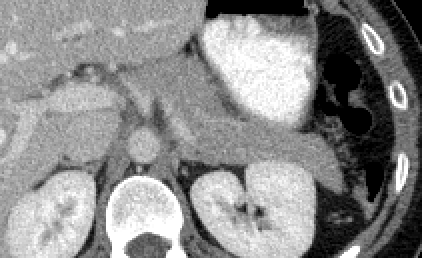
\includegraphics[width=0.205\linewidth]{pancreas_ct_20pct_image.png} &

\includegraphics[width=0.205\linewidth]{pancreas_ct_20pct_gt.png} &

\includegraphics[width=0.205\linewidth]{pancreas_ct_20pct_bcp.png} &

\includegraphics[width=0.205\linewidth]{pancreas_ct_20pct_pem.png} \\
\rotatebox{90}{\scriptsize LA 5\%} &

\includegraphics[width=0.205\linewidth]{la_5pct_image.png} &

\includegraphics[width=0.205\linewidth]{la_5pct_gt.png} &

\includegraphics[width=0.205\linewidth]{la_5pct_bcp.png} &

\includegraphics[width=0.205\linewidth]{la_5pct_pem.png} \\
\rotatebox{90}{\scriptsize LA 10\%} &
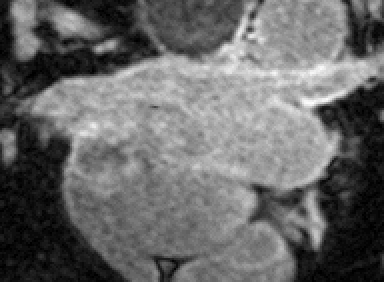
\includegraphics[width=0.205\linewidth]{la_10pct_image.png} &

\includegraphics[width=0.205\linewidth]{la_10pct_gt.png} &

\includegraphics[width=0.205\linewidth]{la_10pct_bcp.png} &

\includegraphics[width=0.205\linewidth]{la_10pct_pem.png} \\
\end{tabular}
\caption{Qualitative results. PEM sharpens the predicted organ boundary relative to the BCP checkpoint on all three configurations, with no labels or pseudo-labels.}
\label{fig:qual}
\end{figure}

\noindent\textbf{Ablations (LA 5\%, one knob at a time).}
Tightening the confidence threshold $\tau$ from $1.0$ to $0.95$ raises the gain from $+0.51$ to $+1.39$ Dice; $\tau=0.999$ discards the shell, while $\tau=0.90$ admits saturated noise. The learning-rate window is narrow: below $10^{-6}$ the collapse-protection triggers within one epoch, and above $5\times10^{-5}$ the boundary is relocated rather than refined. Dice increases monotonically with the epoch budget up to a peak at $E=8$ ($+1.61$); we report the \textit{a priori} $E=5$.

\section{Discussion and Conclusion}
\label{sec:conclusion}
We showed that converged SSL checkpoints leave a structured, boundary-localized residual entropy on their unlabeled data, quantified it with the label-free diagnostic $\rho_f(\tau)$, and exploited it with Post-hoc Entropy Minimization. Whenever $\rho_f(0.99)$ clears the suitability threshold --- as it does for all three released BCP checkpoints, at $0.894$--$0.948$ versus $0.552$ for a supervised-only baseline --- a few minutes of label-free, pseudo-label-free, tuning-free fine-tuning improves the Dice score by $+0.6$ to $+1.4$ points and reduces HD95 by $27$--$43\%$.

PEM has two predictable failure modes, both diagnosable from a single label-free forward pass. When residual entropy is diffuse ($\rho_f\lesssim0.6$, as on the supervised baseline), sharpening reinforces errors. When entropy is already vanishing ($\rho_f\to1$, as on the saturated LA 10\% setting), returns diminish and pseudo-label fine-tuning becomes competitive. Because $\rho_f$ is computed without labels, practitioners can decide in advance whether PEM will help a given checkpoint. A limitation of the present study is that our head-to-head comparison is against BCP, since stronger recent methods release training code only; extending PEM across additional released checkpoints is left to future work.

\bibliographystyle{IEEEtran}
\bibliography{references}

\end{document}
